\documentclass{beamer}
\usepackage[utf8]{inputenc}
\usepackage[spanish]{babel} %Permite definir el idioma del dcumento
%\usepackage[dvips]{epsfig}
%\usepackage[dvips]{graphicx}
\usepackage{url}
\usepackage{ulem}
\usepackage{beamerthemesplit}
\usepackage{moreverb}
\usepackage{color}
\usepackage{listings}
%\usetheme{Warsaw}
\usetheme{Frankfurt}

\title{Presentación CC2}
\subtitle{``Applications of Differential Equations in General Problem Solving''}
\author[R. Fernández/G. Zamora/C. Maureira/]{Rodrigo Fernández\\Gabriel Zamora\\Cristián Maureira}
\date{\today}
%\institution[UTFSM]{Universidad Técnica Federico Santa María}

\begin{document}
\frame
{
	\titlepage
}

\frame
{
	\tableofcontents
}

\section{Introducción}
\frame
{
\frametitle{Introducción}
\framesubtitle{Abstract}
\begin{center}
	1965
\end{center}
\begin{itemize}
	\item Existencia de grandes tipos de problemas relacionados con el procesamiento computacional.
	\item Pueden ser formulados en términos de soluciones numéricas de sistemas de EDO.
	\item Existencia de métodos óptimos para la solución de dichos sistemas.
	\item Propósito, herramientas para procesar dichos problemas.
	\item Punto de vista de programación fácil, debugging, y minimización de tiempo computacional.
\end{itemize}
}

\frame
{
\frametitle{Introducción}
Las clases generales de las ecuaciones tratadas son de la forma:

\begin{eqnarray}
\frac{dy_i}{dx} = f_i (x, y_1, y_2 , \cdots, y_n), \nonumber \\
                \\
y_i (x_0) = y_{i0} ,\ \ \ \ \ \ (i  = 1, 2, 3, \cdots, n). \nonumber
\end{eqnarray}

}

\frame
{
\frametitle{Introducción}
\begin{itemize}
	\item Importancia de éstos problemas (recursos de las bibliotecas de programación).
	\item Subrutinas con distintos niveles de precisión, intervalos de integración, adecuándose al problema.
	\item Eficiencia cercana a la óptima.
	\item Sólo debemos programar los valores derivados (rutinas $\rightarrow$ algoritmos) \textbf{interés}
\end{itemize}
}

\section{Desarrollo}
\subsection{Evaluación de funciones}
\frame
{
\frametitle{Evaluación de funciones}
Tomemos como ejemplo la siguiente función:
$$
	F(x) = x e^{-x} \sum_{n=1}^{\infty}\frac{x^n}{n(n!)}	\ \ \ \ \ \ \ \ (x
\ge 0).  
$$
\begin{enumerate}
	\item Converge lentamente para $x$ grandes.
	\item El número de términos requeridos es del mismo orden que el argumento dado.
	\item Problemas de escalamiento para x muy grandes (límite computacional)
\end{enumerate}
}

\frame
{
\frametitle{Resolución mediante ecuación diferencial}
Por ello, para resolver el problema, es más directo obtener una ecuación diferencial ordinaria que
satisfaga la función $F(x)$:
$$
F'(x) = \{^{\frac{1-x}{x}F(x) + 1 - e^{-x} \ \ \ \ \ \ (x \neq 0),}_{0 \ \ \ \
\ \ \ \ \ \ \ \ \ \ \ \ \ \ \ \ \ \ (x = 0), }
$$
Con $F(0) = 0$.\\
}

\frame
{
\frametitle{Análisis asintótico}
Llegando a una cota superior desde la desde la ecuación diferencial:
$$
F(x) \thicksim 1 + \frac{1!}{x} + \frac{2!}{x^2} + \cdots
$$
}

\frame
{
\frametitle{Análisis asintótico}
$x \in [18,30]$ y N = 50

\begin{center}
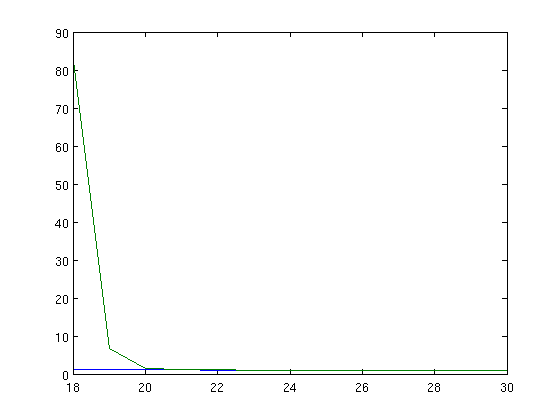
\includegraphics[scale=0.5]{../informe/images/2a.png}
\end{center}
}

\frame
{
\frametitle{Análisis asintótico}
$x \in [20,30]$ y N = 50

\begin{center}
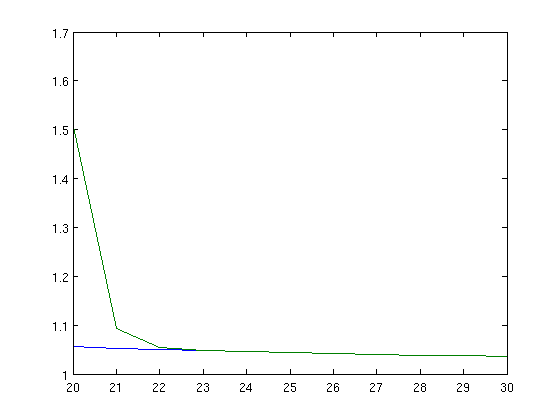
\includegraphics[scale=0.5]{../informe/images/2b.png}
\end{center}
}

\frame
{
\frametitle{Análisis asintótico}
$x \in [22,30]$ y N = 50

\begin{center}
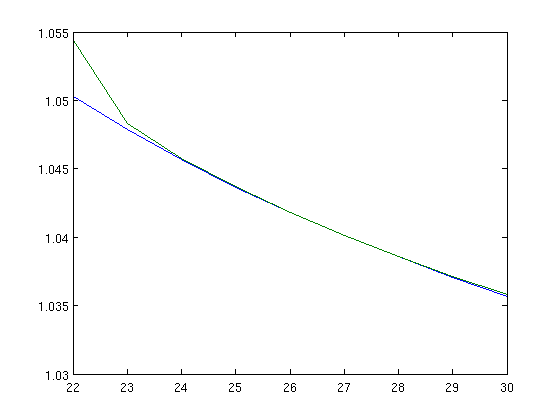
\includegraphics[scale=0.5]{../informe/images/2c.png}
\end{center}
}

\frame
{
\frametitle{Análisis asintótico}
$x \in [24,30]$ y N = 50

\begin{center}
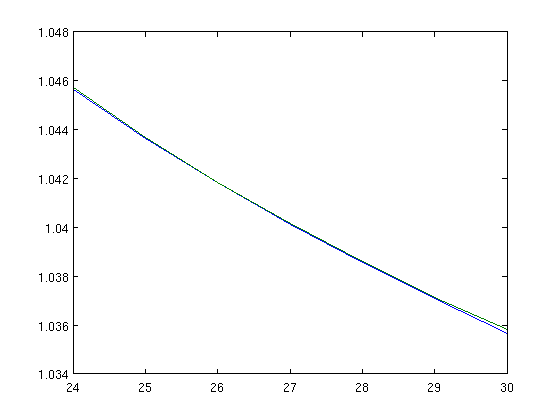
\includegraphics[scale=0.5]{../informe/images/2d.png}
\end{center}
}

\frame
{
\frametitle{Análisis asintótico}
Logrando finalmente darnos cuenta que para valores de x grandes:

$$
F(x) = x e^{-x} \sum_{n=1}^{\infty}\frac{x^n}{n(n!)} \thicksim 1 + \frac{1!}{x} + \frac{2!}{x^2} + \cdots
$$
}


\subsection{Integrales definidas}
\frame
{
\frametitle{Integrales definidas}

$$ I = \int_{a}^{b} f(t) dt $$
}

\frame
{
\frametitle{Integrales definidas}
\framesubtitle{Enfoque estándar}
Realizar la evaluación, seleccionando una fórmula de cuadratura.

\begin{itemize}
	\item Sea $f(x)$ una función continua definida en el intervalo $[a, b]$.
	\item Objetivo, encontrar fórmulas aproximadas para calcular la integral $\int_{a}^{b}f(x) dx$.
	\item En caso de conocer la primitiva $F(x)$ utilizando el Teorema fundamental del cálculo integral:
	 $$\int_{a}^{b}f(x) dx = F(b) - F(a)$$.
	\item Sin embargo no siempre ésto es posible. $f(x) = e^{-x^{2}}$
	\item Ejemplos:
	\begin{itemize}
	        \item Fórmulas de los rectángulos.
	        \item Fórmulas de  los trapecios.
	        \item Método de Simpson.
	        \item etc.
	\end{itemize}
\end{itemize}
}

\frame
{
\frametitle{Integrales definidas}
\framesubtitle{Enfoque estándar}
\begin{itemize}
	\item Volviendo a nuestro tema...
	\item Solución, normalmente realizado conociendo la primitiva $F(x)$ (facilidad de programación).
	\item Entonces, definir una malla de puntos en el intervalo para aplicar la fórmula de cuadratura.
	\item El intervalo de malla seleccionado es casi siempre uniforme y acotado.
	\item Principal dificultad, determinación de un intervalo apropiado de integración. (error)
	\item Errores habituales, mayores derivadas de la función del integrando, $f(t)$. (derivadas altas, poco económica)
	\item Generalmente imposible especificar un intervalo variable de integración.
\end{itemize}
}

\frame
{
\frametitle{Integrales definidas}
\framesubtitle{Enfoque preferido}
Formar una ecuación diferencial mediante la definición de:
$$  I(x) = \int_{a}^{x} f(t) dt $$
y diferenciando
$$  \frac{dI}{dx} = f(x), $$
con $I(a) = 0$, entonces $I(b) = I$
resultado deseado.
}

\frame
{
\frametitle{Integrales definidas}
\framesubtitle{Enfoque preferido}
\begin{itemize}
	\item Sólo una evaluación de la función es necesaria por paso. (en lugar de dos para las derivadas).
	\item Ventajas:
	\begin{itemize}
		\item Rutina de seguimiento continuo monitorea la presición de la integración
		\item y aumenta el intervalo de integración, cuando sea posible.
	\end{itemize}
	\item Vamos construyendo la malla apropiada con sólo una evaluación del integrando por cada paso (precisión)
	\item Un orden de magnitud en el tiempo de cálculo (integrales individuales), dos...
	\item Este enfoque se pueden programar fácilmente y depurado.
	\item Buena rutina asegurará que el punto final (x = b) estará en la malla.
\end{itemize}
}


\subsection{Funciones especiales en el integrando}
\frame
{
\frametitle{Funciones especiales en el integrando}

Misma idea!
Podemos aprovechar ésta técnica para resolver funciones especiales dentro de
una integral.

}
\frame
{
\frametitle{Funciones especiales en el integrando}
\framesubtitle{Aplicación del método 1}

Por ejemplo:

$$
	I	=	\int_0^\infty J_0 (t^2) e^{-t} dt
$$
\textit{(donde $J_0$ es la función regular cilíndrica de Bessel de orden 0)}\\

}
\frame
{
\frametitle{Funciones especiales en el integrando}
\framesubtitle{Aplicación del método 2}
Según lo visto al resolver integrales definidas, podemos hacer:
$$
	\frac{dI}{dx}	=	J_0 (x^2) e^{-x},
$$
con:
$$
	I(0) = 0
$$

Y el resultado deseado de $I(\infty) = I$.\\

}
\frame
{
\frametitle{Funciones especiales en el integrando}
\framesubtitle{Aplicación del método 3}
Ahora, está determinado (creanme) que $J_0(x^2)$ satisface la siguiente
ecuación diferencial ordinaria de segundo orden:
$$
	\frac{d^2y}{dx^2} + (2 - \frac{1}{x}) \frac{dy}{dx} + 4x^2y = 0
$$
con 
$$
	y(0) = 1, \ \ \ \ \ \ \ \ \ \ \ \  y'(0) = 0
$$

}
\frame
{
\frametitle{Funciones especiales en el integrando}
\framesubtitle{Solución}
Simplemente tenemos que resolver el siguiente sistema de ecuaciones
diferenciales:
$$
	\frac{dI}{dx} = y_1 e^{-x}, \ \ \ \ \ \ \ \ \ \ \ \ \ \ \ I(0) = 0,
$$
$$
	\frac{dy_1}{dx} = y_2 ,\ \ \ \ \ \ \ \ \ \ \ \ \ \ \ \ \ \ y_1(0) = 1,
$$
$$
	\frac{dy_2}{dx} = \{^{-(2-\frac{1}{x})y_2-4x^2y_1 \ \ \ \ \ \ (x \neq
0)}_{0 \ \ \ \ \ \ \ \ \ \ \ \ \ \ \ \ \ \ \ \ \ \ (x = 0)}, \ \ \ y_2(0) = 0,
$$
}
\frame
{
\frametitle{Funciones especiales en el integrando}
\framesubtitle{Ventajas}
\begin{enumerate}
	\item Evitamos la necesidad de escribir una subrutina especial.
	\item Exactitud definida y controlada para la integral.
	\item Menos tiempo de computación por cada evaluación de la función.
\end{enumerate}
}

\subsection{Otras aplicaciones}
\frame
{
\frametitle{Otras aplicaciones}
\begin{itemize}
	\item Múltiples integrales definidas.
	\item Ecuaciones diferenciales derivadas en términos de un parámetro del problema.
	\item Ceros en funciones no-lineales (root-tracing)
	\item Equipotenciales, isotérmicos, campos lineales, etc.
	\item Derivadas dadas implícitamente en ecuaciones diferenciales ordinarias.
	\item Integrales oscilatorios
	\item Problemas del valor de dos puntos de la frontera.
	\item Ecuaciones diferenciales parciales parabólicas y hiperbólicas.
	\item Ecuaciones Integrales.
\end{itemize}
}

\section{Conclusiones}
\frame
{
\frametitle{Conclusiones}
\begin{itemize}
	\item La técnica propuesta es interesante y resultó satisfactoria al
probarla computacionalmente.
	\item Como la velocidad y perfomance de los computadores de hoy en día es
ordenes de magnitud más grande que los utilizados en los tiempos de la
publicación, no logramos notar todas las ventajas nombradas por la publicación
estudiada.
	\item Se ha mejorado notablemente el rendimiento de los algoritmos de
resolución de problemáticas de este tipo durante todos estos años, pero no por
eso el tema va a dejar de ser interesante ni va a perder relevancia a futuro.
\end{itemize}

}

\frame
{
\begin{center}
\begin{Huge}\textit{¿Preguntas?}\end{Huge}
\end{center}
}

\end{document}
